\subsubsection{設計パターンとスタイル}

\term{設計パターン}{Design Pattern} は、特定の文脈で繰り返し現れる問題に対する一般的な解決策である。設計パターンは、過去に有効だった設計上の慣用句を共有するための語彙である。

代表的な分類は、生成、構造、振る舞いである。
\begin{itemize}
  \item \textbf{生成パターン}：オブジェクトや部品の生成方法を扱う。ビルダー、ファクトリ、プロトタイプ、シングルトンなどがある。
  \item \textbf{構造パターン}：部品の組み合わせ方を扱う。アダプタ、ブリッジ、コンポジット、デコレータ、ファサード、プロキシなどがある。
  \item \textbf{振る舞いパターン}：責務の分担や相互作用を扱う。コマンド、イテレータ、メディエータ、オブザーバ、状態、戦略、テンプレート、ビジタなどがある。
\end{itemize}

\term{スタイル}{Style} は、より大きな構造の特徴を表す場合に使われることが多い。たとえば、階層化、パイプ・アンド・フィルタ、クライアントサーバ、イベント駆動などは、システム全体または大きな部分の設計方針として現れる。

\begin{figure}[htbp]
\centering
\IfFileExists{assets/fig-ch03-09.png}{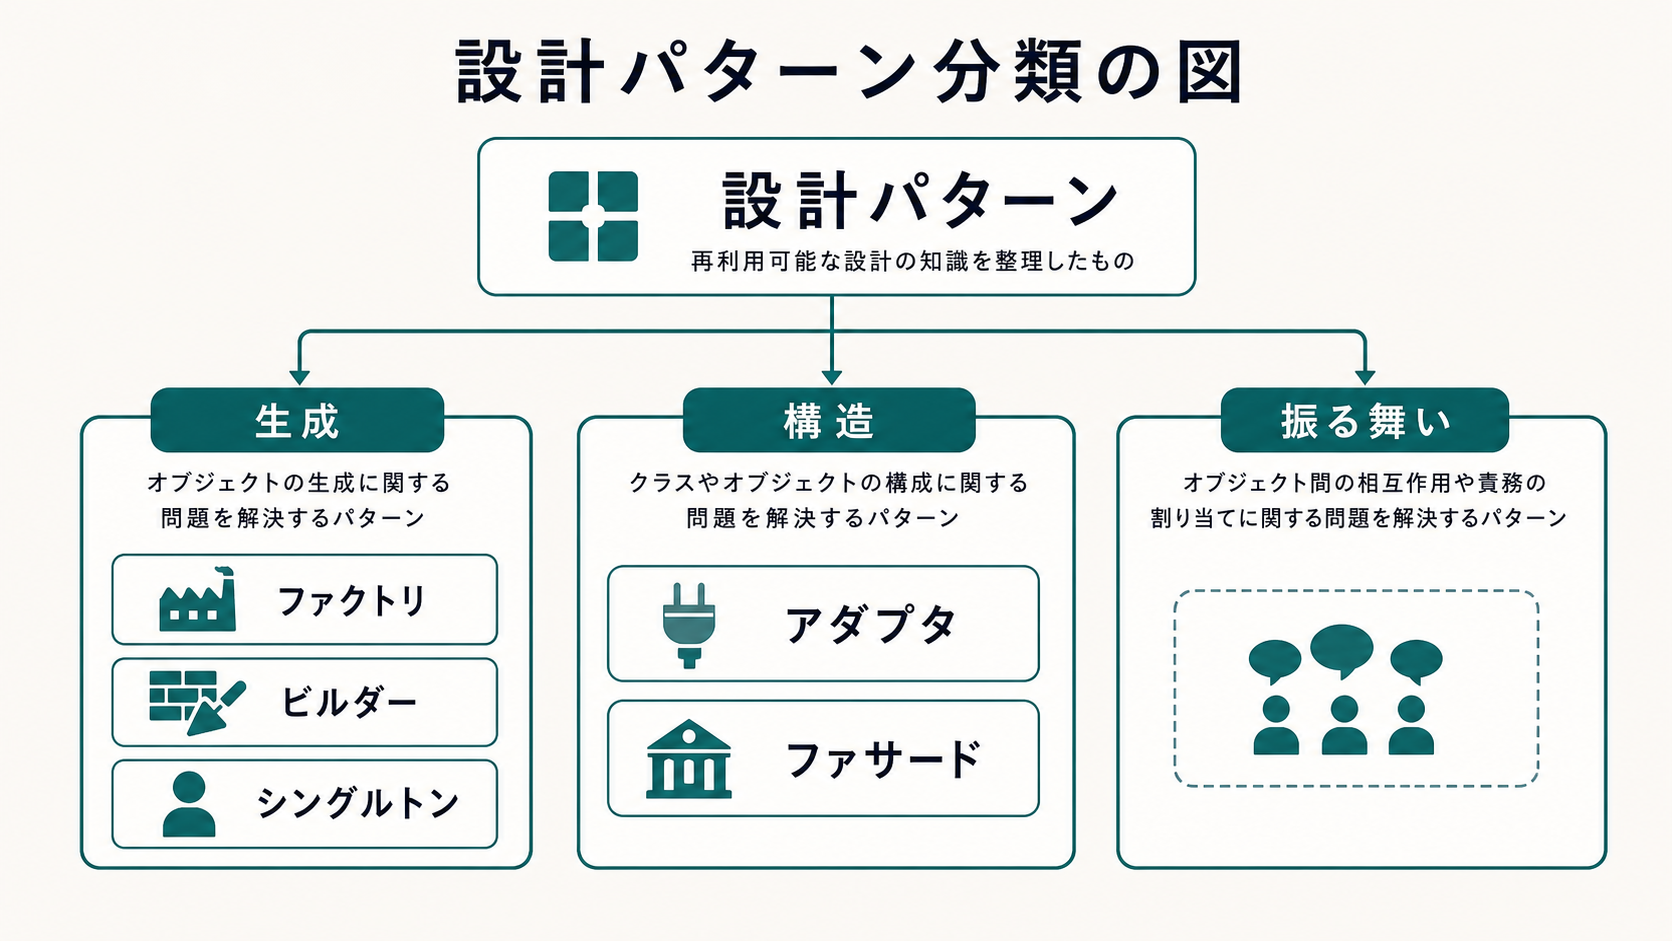
\includegraphics[width=0.96\linewidth]{assets/fig-ch03-09.png}}{\fbox{\parbox[c][48mm][c]{0.9\linewidth}{\centering 画像生成待ち\\設計パターン分類の図}}}
\caption{設計パターン分類の図}
\label{fig:ch03-09}
\end{figure}
